\chapter{Basic definitions of Riemann surfaces}
\label{ch:complex_structure_def}

Roughly speaking, the theory of Riemann surfaces is just the generalization of complex analysis
using ideas from differential geometry:
Just like how a $2$-manifold can be viewed as a collection of patches of the real plane $\RR^2$
smoothly welded together to form a more complicated object,
we take ``pieces'' of the complex plane $\CC$, \emph{analytically} welded together .

We already know that the theory of holomorphic function is very nice --- they're all analytic!
The same amount of rigidity is to be expected here.

In fact, on \emph{compact} Riemann surfaces, the theories are even nicer than the case of
holomorphic functions! For example:
\begin{itemize}
	\ii For two Riemann surfaces $X$ and $Y$ where $Y$ is compact, any meromorphic function $f
	\colon X \to Y$ must in fact be holomorphic i.e. defined everywhere.
	\ii If $X$ is a compact Riemann surface, then a holomorphic function $f \colon X \to \CC$ is
	constant.
	\ii In the same setting as above, furthermore we have that if $g \colon X \to \CC$ is
	meromorphic, then the number of zeros of $g$ is equal to the number of poles of $g$, with
	multiplicity.
\end{itemize}

\begin{remark}[Why do we have these nice properties?]
Roughly speaking, $\CC$ is not compact --- it is isomorphic to the Riemann sphere with a hole
removed. By filling in the hole, we allow meromorphic functions to be extended taking value $\infty$
at places that previously was a pole.
\end{remark}

As an orientable $2$-manifold, we can define the \vocab{genus} of a Riemann surface --- it is a
purely topological concept, yet it is crucially linked to several algebraic invariants
in very surprising ways.
You may have heard of the \emph{elliptic curve} in cryptography --- they also present as a Riemann
surface, and a generalization, \vocab{hyperelliptic curve}, form a family of Riemann surfaces of
arbitrary genus $\geq 2$!

\section{Complex structures}

Recall the definitions in the previous chapters:
\begin{itemize}
	\ii A topological $n$-manifold is a Hausdorff space, with a covering $\{ U_i \}$, each being
	homeomorphic to $\RR^n$.
	\ii A smooth $n$-manifold is a topological $n$-manifold, where all the transition maps are
	smooth.
\end{itemize}
What do they have in common? Seemingly not too much. But essentially, they're all describing the
same philosophy:
\begin{moral}
	We take countably many patches $\{ U_i \}$, and weld them together while keeping the underlying
	structure.
\end{moral}

Here, a topological manifold has a \emph{topological structure}, and a smooth manifold has a
\emph{smooth structure}. In a similar manner, a complex manifold has a \emph{complex structure}.

What do we mean by ``structure'' here?

First, a topological structure is familiar to you --- it's just a topology.
Formally, the topology is defined by the collection of open sets, but the actual \emph{meaning} of a
topological structure dictates:
\begin{itemize}
	\ii whether a set is considered open or closed,
	\ii whether a sequence of points converge to a given point,
	\ii whether a map $X \to Y$ or $Y \to X$ is continuous (given $Y$ is another topological space),
	\ii etc.
\end{itemize}

Given a topological $n$-manifold with an existing (Hausdorff) topology on it, we can tell whether a
local chart \emph{respects the topological structure}; in other words, is a homeomorphism.
\begin{example}[$(0, 2)$ is a topological $1$-manifold]
	The open interval $(0, 2)$ included in $\RR$ can be considered a topological manifold.
	\begin{center}
		\begin{asy}
			size(8cm);
			draw((0, 5)--(8, 5), black+2);
			dotfactor*=2;

			void drawsegment(pair a, pair b, Label L, pen p=defaultpen){
				draw(a--b, p); opendot(a, p); opendot(b, p);
				label((a+b)/2, L, S, p);
			}

			var a=(3, 4), b=(5, 4);
			draw(a--b, black+2); opendot(a); opendot(b);

			label((4, 4.5), rotate(90)*Label("$\subseteq$"));
			label((3, 5), "$0$", S);
			label((5, 5), "$2$", S);
			var E1l=(1, 1), E2l=(5.7, 1), E2r=E2l+(1.3, 0);
			drawsegment(E1l,(3, 1), "$E_1$", blue);
			drawsegment(E2l,E2r, "$E_2$", red);

			var v=(2/6, 0);
			for(int i=0; i<=6;++i){
				draw(a+i*v--E1l+i*v, blue, Arrow, Margin(2));
				draw(a+i*v--E2l+(i<=3 ? i*v: 3*v+(i-3)*(0.1, 0)), red, Arrow, Margin(2));
			}
			label((8, 5), "$\mathbb{R}$", NW);

			label((a+E1l)/2, "$\phi_1$", blue, align=NW);
			label((b+E2r)/2, "$\phi_2$", red, align=NE);
		\end{asy}
	\end{center}
	Two possible charts for the space, $\phi_1$ and $\phi_2$, are shown.

	Their formulas are $\phi_1 \colon (0, 2) \to (0, 2), \phi_1(x) = x$ and $\phi_2 \colon (0, 2)
	\to (0, 1.3), \phi_2(x) = x + 0.35 \cdot (1-x-\abs{1-x})$.
\end{example}

In the example above, you may notice that, even though the chart $\phi_2$ is a homeomorphism,
it doesn't look \emph{smooth}. So, you want to define a smooth $2$-manifold as something like:
\begin{quote}
	A surface $S \subseteq \RR^3$ is a smooth $2$-manifold if, for each $p \in S$, there exists an
	open neighborhood $V \subseteq S$ that is diffeomorphic to $E \subseteq \RR^2$.
\end{quote}
In fact, this is the actual definition in classical differential geometry --- of course, this isn't
completely general, for instance, we know that the Klein bottle cannot be embedded into $\RR^3$.

So, why didn't we define something like this in \Cref{def:smooth_manif}?
The problem is, the concept of a diffeomorphism isn't defined on a Hausdorff topological space ---
in fact it can't be defined, right in the example above, you can see a homeomorphism that is not
a diffeomorphism --- in other words, a topological space can be assigned different \emph{smooth
structures}.

So, the essence of what the definition \Cref{def:smooth_manif} is doing is, it implicitly defines
what a \emph{smooth structure} mean, by inducing the smooth structure from each patch $E_i \subseteq
\RR^n$ to the topological space $M$.
The condition that the transition functions need to be smooth is, of course, to ensure that the
smooth structures on $M$ induced by different $\phi_i$ are the same.

In completely the same way, we could have replaced \Cref{def:topological_manif} by:
\begin{quote}
	A topological $n$-manifold $M$ is a set with a collection of subsets $\{ U_i \}$ that covers
	$M$, for each $U_i$ there is a bijective map from it to a subset of $\RR^n$, say
	\[ \phi_i \colon U_i \to E_i \subseteq \RR^n \]
	where each $E_i$ is an open subset of $\RR^n$, satisfying that all the transition maps are
	topological homeomorphisms.
\end{quote}

Here, the $\phi_i$ are ``set isomorphisms'' and plays a similar role as the homeomorphisms in
\Cref{def:smooth_manif}, and the topological space structure is
similarly induced from the patches $E_i$.

\begin{example}[$(0, 2)$ is a smooth $1$-manifold]
	Just as above, the open interval $(0, 2)$ included in $\RR$ can also be considered a
	smooth manifold.
	\begin{center}
		\begin{asy}
			size(8cm);
			draw((0, 5)--(8, 5), black+2);
			dotfactor*=2;

			void drawsegment(pair a, pair b, Label L, pen p=defaultpen){
				draw(a--b, p); opendot(a, p); opendot(b, p);
				label((a+b)/2, L, S, p);
			}

			var a=(3, 4), b=(5, 4);
			draw(a--b, black+2); opendot(a); opendot(b);

			label((4, 4.5), rotate(90)*Label("$\subseteq$"));
			label((3, 5), "$0$", S);
			label((5, 5), "$2$", S);

			real phi1(real x){return x;}
			real phi2(real x){return x+(x>1 ? exp(-1/(x-1)): 0);}

			var E1l=(1, 1), E2l=(7.3-phi2(2), 1);
			drawsegment(E1l,E1l+phi1(2), "$E_1$", blue);
			drawsegment(E2l,E2l+phi2(2), "$E_2$", red);

			for(int i=0; i<=6;++i){
				var x=i/3;
				draw(a+x*E--E1l+phi1(x)*E, blue, Arrow, Margin(2));
				draw(a+x*E--E2l+phi2(x)*E, red, Arrow, Margin(2));
			}
			label((8, 5), "$\mathbb{R}$", NW);

			label((a+E1l)/2, "$\phi_1$", blue, align=NW);
			label((b+E2l+phi2(2))/2, "$\phi_2$", red, align=NE);
		\end{asy}
	\end{center}
	This time around, $\phi_1$ is the same as above, but
	$\phi_2 \colon (0, 2) \to (0, 2 + \frac{1}{e})$ is defined by
	\[ \phi_2(x) = \begin{cases}
		x & \text{if } x \leq 1 \\
		x + e^{-1/(x-1)} & \text{otherwise}.
	\end{cases} \]

	Because all of $\phi_1$, $\phi_2$, and their inverses are smooth functions, the transition maps
	$\phi_1 \circ \phi_2\inv$ and $\phi_2 \circ \phi_1\inv$ are thus smooth, satisfying
	the hypothesis of \Cref{def:smooth_manif}.
\end{example}

You should take a moment to think through this idea --- because smooth functions on $\RR^n$ are so
natural, it's easy to forget that a smooth manifold carries more structure than just the topology.

Once again, as we have seen in the example above, $\RR^n$ has more structure than just being smooth
--- it has an \emph{analytic structure}. The chart $\phi_2$ does not preserve this structure.

So, for Riemann surface, we will just have:
\begin{moral}
	A Riemann surface is a smooth (real) $2$-manifold which locally looks like $\CC$, and carries an
	\emph{complex-smooth structure}.
\end{moral}

Of course, by the miracle of complex analysis --- holomorphic functions are analytic! --- this is
equivalent to stating that a Riemann surface carries a complex-analytic structure.

\section{Riemann surface}
\prototype{The Riemann sphere, or any open subset of $\CC$ such as $\{ z \in \CC \mid |z| < 1 \}$.}

From the motivation above, the definition of a Riemann surface naturally falls out:
\begin{definition}[Riemann surface]
	A \vocab{Riemann surface} $X$ is a second countable connected Hausdorff space with an open cover
	$\{ U_i \}$ of countably many sets homeomorphic to open subsets of $\CC$, say by homeomorphisms
	\[ \phi_i \colon U_i \taking\cong E_i \subseteq \CC \]
	such that the \vocab{transition maps} $\phi_{ij}$ defined by
	\[
		\phi_{ij} \colon E_i \cap \phi_i\im(U_i \cap U_j)
		\taking{\phi_i\inv}
		U_i \cap U_j
		\taking{\phi_j} E_j \cap \phi_j\im(U_i \cap U_j).
	\]
	are analytic functions.
	Each $\phi_i$ is called a \vocab{complex chart}, and together they form a \vocab{complex atlas}.
\end{definition}

We say that the complex atlas gives the Hausdorff space a \vocab{complex structure}.
Thus, in other words, a Riemann surface is a (second countable, connected, Hausdorff) topological
space with a complex structure.

\cite{ref:miranda} has an alternative definition, by a maximal complex atlas. Both definitions are the same,
but in practice, it's easier to specify finitely many complex charts than specifying infinitely many
ones.

A complex chart $U_i \to E_i$ should be think of as giving a \vocab{local coordinate} on $U_i$.
Formally:
\begin{definition}
	For a point $p \in X$, open set $U \subseteq X$ and complex chart $\phi \colon U \to \CC$,
	let $z = \phi(x)$ for each $x \in U$, we call $z$ a \vocab{local coordinate}.
	We say that the local coordinate is \vocab{centered} at $p$ if $\phi(p) = 0$.
\end{definition}

\section{Complex manifold}
Analogously to the definition of a real $n$-manifold, we can define a complex manifold.
Just as above, the structure has much more rigidity than a smooth surface.

\begin{definition}[Complex $n$-manifold]
	A \vocab{complex $n$-manifold} is a Hausdorff space with an open cover $\{ U_i \}$ of countably
	many sets homeomorphic to open subsets of $\CC^n$, say by homeomorphisms
	\[ \phi_i \colon U_i \taking\cong E_i \subseteq \CC^n \]
	such that the \vocab{transition maps} $\phi_{ij}$ are analytic functions.
\end{definition}
Of course, a complex $n$-manifold is naturally a smooth (real) $2n$-manifold.

\section{Examples of Riemann surfaces}

In this chapter, several examples will be given.
\begin{example}[Open subsets of $\CC$]
	Any connected open subset $U \subseteq \CC$ is a Riemann surface.
	\begin{center}
		\begin{asy}
			size(6cm);
			graph.xaxis(xmin=-3, xmax=3);
			graph.yaxis(ymin=-3, ymax=3);
			filldraw(
				(1, 2)..(2, 2)..(1, 3)..(-2, 2)..(-2, -2)..(1, -1)..(1, 0)..(0, 1)..cycle,
				opacity(0.1)+lightcyan, heavycyan);
			label("$U$", (1, 0), NE);
		\end{asy}
	\end{center}

	This is a boring example (the whole thing can be defined without any welding), but let's go on.
\end{example}

\begin{example}[The Riemann sphere]
	\label{ex:riemann_sphere}
	The Riemann sphere $\CC_\infty$, as a smooth $2$-manifold, is just a sphere.
	\begin{center}
		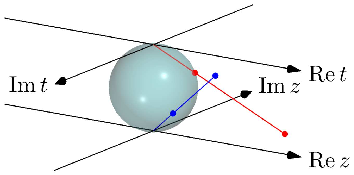
\includegraphics{3dfigures/pdf/riemsphere.pdf}
	\end{center}
	Its complex structure is defined as follows:

	Embed the sphere in $\RR^3$ such that $N = (0, 0, 1)$ and $S = (0, 0, 0)$ are two antipodal
	points.

	Let $E_1$ be the $xy$-plane, and let $E_2$ be the set of points with $z = 1$.

	Then, let $\phi_1 \colon \CC_\infty \setminus \{ N \} \to E_1$ be the stereographic projection
	from the sphere (except the point $N$) to $E_1$ through the point $N$,
	and let $\phi_2 \colon \CC_\infty \setminus \{ S \} \to E_2$ be the stereographic projection
	from the sphere (except the point $S$) to $E_2$ through the point $S$.

	We think of $E_1$ and $E_2$ as copies of the complex plane embedded in $\RR^3$ by $z \mapsto
	(\Re z, \Im z, 0) \in E_1$ and $t \mapsto (\Re t, -\Im t, 1) \in E_2$.
	Then $\phi_1$ and $\phi_2$ are complex charts for $\CC_\infty$.

	The domain of $\phi_1$ and $\phi_2$ covers $\CC_\infty$.
	To make $\CC_\infty$ into a complex manifold, we must ensure that the complex structure induced
	by $\phi_1$ and $\phi_2$ are the same --- indeed, over any open set $U$ that contains neither
	$N$ nor $S$, the projections are related by $\phi_1(p) = \frac{1}{\phi_2(p)}$ for all $p \in U$.

	This also explains why the minus sign is needed in $t \mapsto (\Re t, -\Im t, 1)$ ---
	otherwise, the projections will be related by
	$\phi_1(p) = \frac{1}{\left(\ol{\phi_2(p)}\right)}$, which is not analytic.

	We can think of the Riemann sphere as the result of welding two copies of $\CC$ together in order
	to ``fill in'' the missing point $\infty$.
\end{example}

In the example above, the local coordinate given by $\phi_1$ is centered at $S$, and the local
coordinate given by $\phi_2$ is centered at $N$.
The point $\phi_1\inv(4)$ would have local coordinate $z = 4$ under the chart $\phi_1$, and
local coordinate $t = \frac{1}{4}$ under the chart $\phi_2$.

\begin{example}[The complex torus]
	Let $L$ be the set $\ZZ[i]$ of complex numbers with both real and imaginary parts of $\CC$.
	Then $L$ forms an additive subgroup of $\CC$.

	Consider the quotient $\CC/L$. The quotient map $\CC \to \CC/L$ induces a natural complex
	structure on $\CC/L$.

	\begin{center}
		\begin{asy}
			size(6cm);

			filldraw(unitsquare, opacity(0.3)+lightcyan, heavycyan);
			draw((-3.5, 0) -- (3.5, 0), Arrow);
			draw((0, -3.5) -- (0, 3.5), Arrow);
			for(int x=-3; x<=3; ++x) for(int y=-3; y<=3; ++y) dot((x, y), blue);
			label((3, 3), "$L$", NE, blue);

			draw((0.5, -3.5)--(0.5, -4.8), Arrow);
			filldraw(shift(0, -6)*unitsquare, opacity(0.3)+lightcyan, heavycyan);
			label((0, -6)+(1, 0.7), "$\mathbb{C}/L$", E, heavycyan);
		\end{asy}
	\end{center}

	Here we draw $\CC/L$ as a square, but you should imagine that the top and bottom edge, as well
	as the left and right edges, are smoothly welded together.

	For each small patch of the torus, we can isomorphically map it to $\CC$ by taking a suitable
	component of the preimage of the quotient map --- the different choices of the projection are
	related by transition functions $\phi_{ij}(x) = x + a$ for $a \in L$, this is analytic.

	The complex torus is compact, thus any holomorphic function on $\CC/L$ is constant. Meromorphic
	functions are more interesting, and also difficult to construct.
\end{example}

And some non-examples.
\begin{example}
	The disjoint union of two Riemann spheres is not a Riemann surface, because it is not connected.
\end{example}
The condition that a Riemann surface must be connected is merely a technical condition such that
theorems are nice --- we don't lose much by requiring this, because any topological space with a
complex structure can be broken down into disjoint union of Riemann surfaces, one for each connected
component.
